\section{Experiments}
\label{sec:experiments}

\subsection{Protocol and claim gates}
\paragraph{Models, data, and interventions.}
We evaluate the official VGGT~\cite{wang2025vggt} and
DUSt3R~\cite{wang2024dust3r} checkpoints without fine-tuning.  ETH3D
\cite{schops2017eth3d} uses four deterministic raw views from each of all 13
training scenes, with raw scan-supported depth.  DTU~\cite{jensen2014large} is
held out until transforms, scores, thresholds, and qualitative scenes are
frozen; it uses the standard 22 MVS evaluation scans, pixelNeRF's three view
indices 22/25/28~\cite{yu2021pixelnerf}, and lighting condition 3.  The common
11-variant matrix contains identity; center, shared off-center, and independent
off-center crops at 90/75/60\% retention; and square letterbox.  This gives 286
ETH3D and 484 DTU GT evaluations.  DUSt3R uses complete symmetrized pairs and
300 optimizer iterations.

Every record receives relative pose and intrinsic evaluation.  ETH3D also uses
affine-aware raw depth and camera-pose-aligned point maps.  DTU point maps are
evaluated for the four frozen primary variants using the official observation
mask and ground plane, strict 20-mm directional filters, deterministic 0.2-mm
voxelization, and a 100k-point cap.  Because these are three-view point maps
rather than an MVS submission, we call this the \method DTU point metric, not a
leaderboard score.  Empty directional sets are undefined, never zero-filled.

\paragraph{Statistics and chronology.}
All comparisons are paired by model, scene, views, and transform.  We report
scene medians with deterministic 95\% percentile intervals from 10,000 scene
bootstrap replicates (seed 17).  A family crosses the mechanism gate when a
paired rotation increase exceeds \SI{2}{\degree} or depth AbsRel increases by
0.05.  DTU is opened only after the mechanism design and reliability score are
fixed.  The support-preserving control is registered after seeing ETH3D crop
results but before any of its own outcomes and before DTU GT.  It is therefore
prospective for the control and DTU, not retrospectively preregistered ETH3D
evidence.  A preceding three-scene diagnostic and exact identity repeat were
used only to validate the pipeline; no diagnostic disagreement is presented as
GT accuracy.

\subsection{A two-model, two-dataset failure}
Table~\ref{tab:cross-dataset} gives the main result.  Independent 75\% crops
increase median rotation error for both models on both datasets: VGGT by
\SI{4.61}{\degree} on ETH3D (95\% CI [3.13, 6.17]) and
\SI{5.19}{\degree} on DTU ([4.44, 6.02]); DUSt3R by
\SI{4.52}{\degree} ([2.13, 5.72]) and \SI{2.96}{\degree}
([1.69, 4.08]).  Translation-direction increases are 9.49/10.99 degrees on
ETH3D and 3.63/2.60 degrees on DTU for VGGT/DUSt3R.  The normalized
principal-point delta is 3.71/3.69 percentage points on ETH3D and 4.39 points
for both models on DTU, matching the intervention's camera mechanism.

On ETH3D the same crop increases depth AbsRel by 2.30 and 1.64 percentage
points and completeness by 369 and \SI{416}{\milli\meter}; all four intervals
exclude zero.  VGGT DTU point accuracy and completeness rise by 2.74
([1.30, 6.02]) and \SI{2.50}{\milli\meter} ([1.77, 4.66]).  The DUSt3R DTU
camera result is complete, but one or two scenes per point direction have no
valid strict-filter pair; the registered complete-design aggregate is therefore
undefined instead of being computed on a favorable subset.

\begin{table*}[t]
  \centering
  \caption{Two-model, two-dataset GT result.  Rotation entries are
  \emph{absolute error / paired increase from identity}; Shared is the paired
  rotation increase for one off-center 75\% window reused across views. Point
  columns are paired accuracy/completeness increases in millimeters. Medians
  are across scenes; models and datasets are never pooled.}
  \label{tab:cross-dataset}
  \setlength{\tabcolsep}{6pt}
  \begin{tabular}{llrrrr}
    \toprule
    Model & Dataset & Identity rot. & Independent 75\% rot. & Shared 75\% & Point A/C $\Delta$ \\
    \midrule
    VGGT   & ETH3D & 0.81 & 5.27 / +4.61 & +2.38 & +259 / +369 \\
    DUSt3R & ETH3D & 1.28 & 5.67 / +4.52 & +2.18 & +252 / +416 \\
    VGGT   & DTU   & 0.46 & 5.58 / +5.19 & +2.01 & +2.74 / +2.50 \\
    DUSt3R & DTU   & 2.05 & 5.45 / +2.96 & +1.95 & undefined$^\dagger$ \\
    \bottomrule
  \end{tabular}
  \\[1pt]
  {\footnotesize $^\dagger$Strict-filter missingness prevents a complete 22-scene point bootstrap; no value is imputed.}
\end{table*}

\paragraph{Severity and crop scope.}
Figure~\ref{fig:mechanism-severity} shows all four model--dataset aggregates.
Independent crops are monotone as retention decreases and cross two degrees at
75\% and 60\% everywhere.  Shared off-center crops also form a replicated
failure family: at 60\%, their deltas are 3.71/3.30 degrees on ETH3D and
3.76/4.59 degrees on DTU for VGGT/DUSt3R.  At matched severity the independent
window is generally worse, isolating view dependence as an amplifier.  Center
crops never cross the gate, and symmetric letterbox stays below it.  Thus the
registered two-family, two-dataset mechanism gate passes without pooling
models or substituting depth for pose.

\begin{figure*}[t]
  \centering
  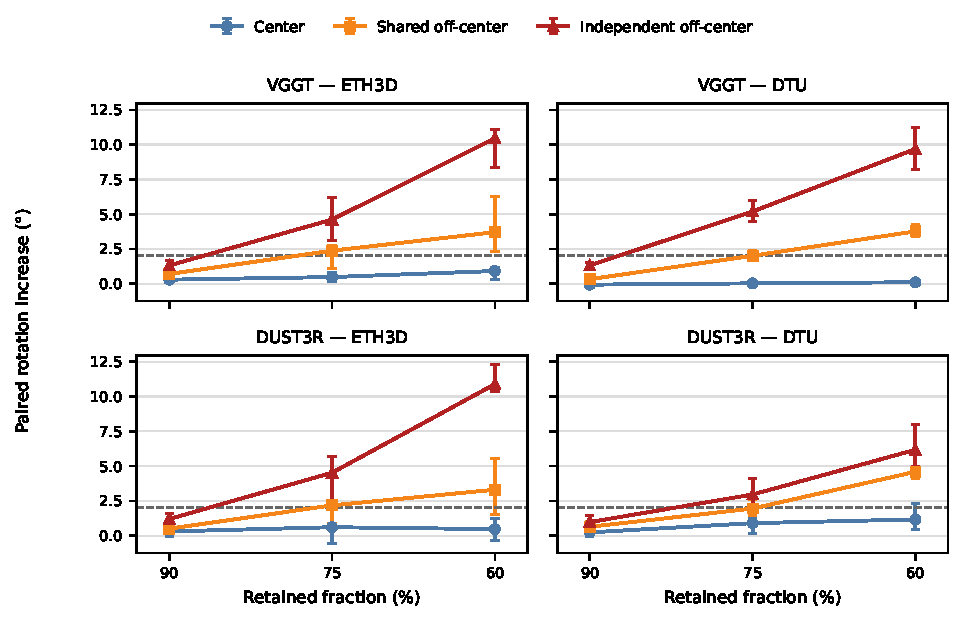
\includegraphics[width=0.86\textwidth]{figures/mechanism_severity.pdf}
  \caption{Paired rotation increase versus retained fraction.  Points are
  scene medians; bars are 95\% scene-bootstrap intervals; the dashed line is
  the frozen \SI{2}{\degree} gate.  Independent and shared off-center families
  cross on both datasets, while center crops remain below threshold.}
  \label{fig:mechanism-severity}
\end{figure*}

\subsection{Support-preserving coordinate control}
Cropping changes coordinates and visible support together.  To test whether
support loss is necessary, we place every decoded source RGB pixel byte-for-byte
and at scale one on the same square canvas.  Centered, shared-edge, and
independently sampled edge placements have identical source pixels, output
shape, and black-padding count; an audit binds the centered image bytewise to
the main letterbox control.  Only pixel position changes.

Table~\ref{tab:support-control} is the most direct causal result.  Independent
placement adds 13.97/10.90 degrees on ETH3D and 10.78/5.69 degrees on DTU for
VGGT/DUSt3R; every confidence interval lies far above two degrees.  Shared edge
placement is smaller but nonzero.  Support loss is therefore not required for
the failure: absolute and view-relative canvas coordinates affect predicted
cameras even when RGB support is preserved exactly.

\begin{table}[t]
  \centering
  \caption{Support-preserving control: paired rotation increase from centered
  letterbox.  Independent entries include 95\% CIs.}
  \label{tab:support-control}
  \setlength{\tabcolsep}{3.5pt}
  \begin{tabular}{llrr}
    \toprule
    Model & Data & Shared edge & Independent edge \\
    \midrule
    VGGT   & ETH3D & 5.17 & 13.97 [9.80, 15.33] \\
    DUSt3R & ETH3D & 3.87 & 10.90 [8.11, 16.28] \\
    VGGT   & DTU   & 1.74 & 10.78 [10.02, 11.30] \\
    DUSt3R & DTU   & 2.16 & 5.69 [4.98, 5.93] \\
    \bottomrule
  \end{tabular}
\end{table}

\subsection{Canonical-camera repair}
For error $E$, gap recovery is
$\left(E_{\rm crop}-E_{\rm repair}\right)/
 \left(E_{\rm crop}-E_{\rm identity}\right)$.
The frozen promotion rule requires at least 0.30 rotation recovery and less
than 2\% identity degradation.  Table~\ref{tab:repair} shows that neutral-gray
canonicalization passes on both datasets and models.  On held-out DTU it
recovers 0.941 of the VGGT rotation gap (95\% CI [0.888, 1.042]) and 0.767 of
the DUSt3R gap ([0.421, 1.251]); both lower bounds exceed 0.30.  Identity
predictions repeat byte-exactly, so measured clean rotation cost is zero.

The supported claim remains orientation-specific.  On ETH3D every registered
fill worsens depth; neutral-gray recovery is $-1.38$ for VGGT and $-12.61$ for
DUSt3R.  On DTU, VGGT point completeness recovery is 0.915 ([0.538, 1.296]),
but accuracy's lower bound is 0.256 and DUSt3R lacks a complete point aggregate.
A three-fill selector costs three model runs, slightly improves ETH3D VGGT,
and ties the DUSt3R neutral baseline; it fails the multi-model gate and is not
promoted.

\begin{table}[t]
  \centering
  \caption{Canonical repair of independent 75\% crops. Rotation columns are
  absolute GT error in degrees; Rec. is paired gap recovery. Clean cost is zero
  in all rows.}
  \label{tab:repair}
  \setlength{\tabcolsep}{3.5pt}
  \begin{tabular}{llrrrr}
    \toprule
    Model & Data & Identity & Crop & Repair & Rec. \\
    \midrule
    VGGT   & ETH3D & 0.805 & 5.274 & 1.449 & 0.966 \\
    DUSt3R & ETH3D & 1.276 & 5.667 & 2.934 & 0.558 \\
    VGGT   & DTU   & 0.459 & 5.581 & 0.499 & 0.941 \\
    DUSt3R & DTU   & 2.051 & 5.448 & 3.366 & 0.767 \\
    \bottomrule
  \end{tabular}
\end{table}

\begin{figure*}[t]
  \centering
  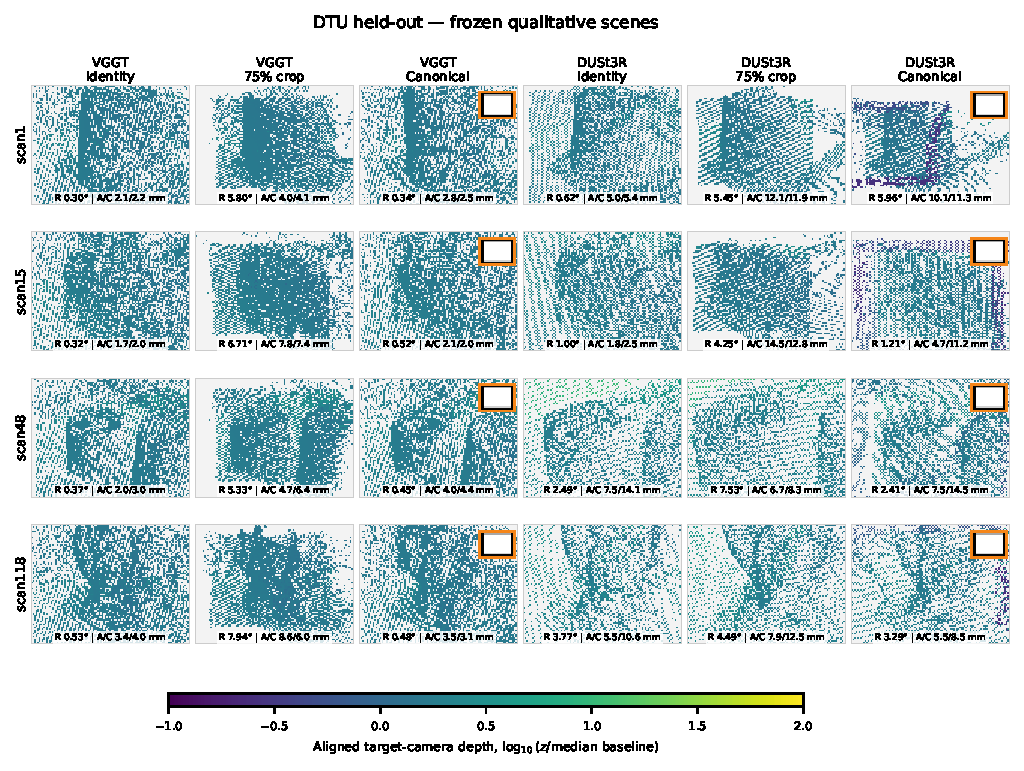
\includegraphics[width=\textwidth]{figures/qualitative_dtu.pdf}
  \caption{Outcome-independent DTU qualitative set frozen before model outputs.
  We project aligned point maps into the first target camera with a shared depth
  scale and color range.  Each panel reports rotation and point
  accuracy/completeness; orange insets show canonical validity masks.  All four
  scenes and both models are retained, including the mixed DUSt3R repairs.}
  \label{fig:qualitative-dtu}
\end{figure*}

\subsection{Held-out failure detection}
We freeze four DTU cases per scene and label a failure when median rotation
error is strictly greater than \SI{2}{\degree}.  AUROC uses average ranks for
ties; risk--coverage adds complete tie blocks; intervals resample scenes as
clusters.  Table~\ref{tab:reliability} and
Fig.~\ref{fig:risk-coverage} show that disagreement passes the absolute 0.75
AUROC gate for both models.  VGGT is nearly separable (0.998) and its excess
AURC is one tenth of the native score.  DUSt3R reaches 0.855, but its native
score has the identical AUROC and a slightly worse AURC.  The detector is
therefore useful across models, while the stronger claim that it universally
beats native uncertainty fails.

\begin{table}[t]
  \centering
  \caption{Held-out DTU reliability. D/N are disagreement/native; O is oracle.
  AUROC intervals use 10k scene-cluster replicates. AURC is mean rotation risk;
  lower is better.}
  \label{tab:reliability}
  \setlength{\tabcolsep}{3pt}
  \resizebox{\columnwidth}{!}{%
  \begin{tabular}{lrrrr}
    \toprule
    Model & Failures & D AUROC & N AUROC & AURC D/N/O \\
    \midrule
    VGGT & 23/88 & .998 [.990,1] & .647 [.576,.722] & .678/1.259/.610 \\
    DUSt3R & 59/88 & .855 [.732,.949] & .855 [.743,.933] & 2.472/2.561/1.820 \\
    \bottomrule
  \end{tabular}%
  }
\end{table}

\begin{figure*}[t]
  \centering
  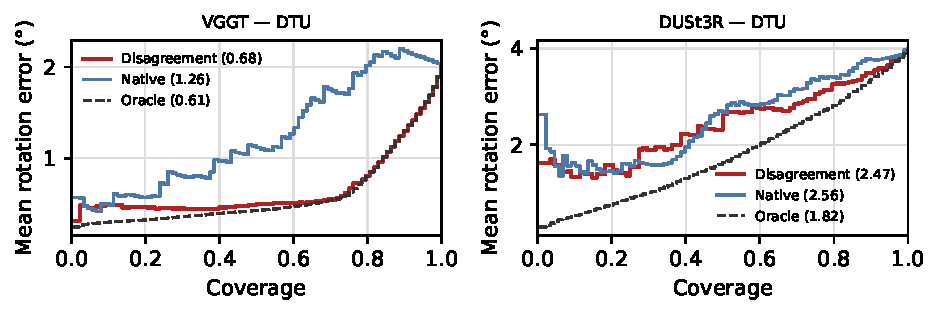
\includegraphics[width=0.80\textwidth]{figures/dtu_risk_coverage.pdf}
  \caption{Held-out DTU risk--coverage with complete tie blocks.  Legend values
  are AURC.  Disagreement strongly improves VGGT selection; on DUSt3R it is
  useful but only slightly better in AURC and equal in AUROC to native
  uncertainty.}
  \label{fig:risk-coverage}
\end{figure*}

\subsection{Compute and reproducibility}
Table~\ref{tab:compute} separates model-only time from end-to-end time and
one-time loading.  DTU end-to-end includes image IO, hashing, model
pre/postprocessing, and compressed prediction writes, but excludes model load
and final metadata write.  Canonicalizing one corrupted DTU scene takes a
median 0.794 seconds before inference; the repaired model run has essentially
the same cost as a direct run.  Legacy ETH3D metadata predates the end-to-end
boundary, so that field is explicitly unavailable rather than reconstructed.

All 770 main records, 210 support-control records, and 88 repair records have
complete-design checks and source/config hashes.  The committed evidence bundle
copies 833 lightweight files and records SHA-256 hashes for all 782 large DTU
and support-control predictions without placing them in Git.

\begin{table}[t]
  \centering
  \caption{Per-scene compute on RTX 5090. Model/E2E are median seconds; VRAM is
  maximum GiB. ETH3D E2E is unavailable under the legacy timing schema.}
  \label{tab:compute}
  \setlength{\tabcolsep}{5pt}
  \begin{tabular}{llrrr}
    \toprule
    Model & Data & Model & E2E & VRAM \\
    \midrule
    VGGT   & ETH3D & 0.155 & --    & 5.79 \\
    DUSt3R & ETH3D & 4.799 & --    & 2.59 \\
    VGGT   & DTU   & 0.142 & 0.719 & 5.49 \\
    DUSt3R & DTU   & 4.464 & 5.222 & 2.59 \\
    \bottomrule
  \end{tabular}
\end{table}
